\chapter{Noyau de l'application}

	L'objectif de l'application finale est de fournir un gestionnaire de tâches (\emph{todolist}) proposant à l'utilisateur des fonctionnalités avancées. Il nous était justement demandé d'implémenter les fonctionnalités suivantes :
	\begin{itemize}
		\item Ajout/Modification/Suppression de tâches, de listes de tâches, et de listes de listes de tâches ;
		\item Gestion de templates de listes de tâches ;
		\item Préconditions à la validation de tâches ;
		\item Permettre d'ordonner les listes ;
		\item Gestion de dates limites (\emph{deadlines}) à une tâche ou à une liste, et pouvant être relatives à une autre date ;
		\item Sauvegarde et chargement XML.
	\end{itemize}

	\section{Analyse}
	
		À partir des fonctionnalités qui nous étaient demandées, nous avons commencé à réfléchir à une conception du noyau de l'application qui nous permettrait une développement rapide au vu du peu de temps qui nous était imparti.\\
		
		À haut niveau, nous avons décidé de manipuler deux principaux types d'objets : les listes et les tâches. Un conteneur, que nous avons appelé modèle, nous servira de référence pour accéder au noyau de l'application. Il s'agit d'une sorte de porte d'accès aux données, un objet contenant une liste des listes ajoutées par l'utilisateur (vector<List*>), et proposant une interface complète permettant au développeur d'agir sur le noyau entier. Un objet liste est lui composé d'une liste de listes (vector<List*> qui seront en fait des sous-listes), et d'une liste de tâches (vector<Task*>). Cette conception nous permet ainsi de bénéficier d'un niveau de profondeur infini. L'ordonnancement des listes sera gérée à plus bas niveau, au niveau de la structure utilisée (vector).
		Nous aurions pu n'utiliser qu'un seul objet Tâche qui aurait les propriétés de nos deux objets, ce qui aurait peut-être permi de simplifier la maintenance de l'application mais qui nous aurait fait perdre du temps sur le développement étant donné l'IHM que nous avons prototypée (différenciation claire des listes et des tâches, voir plus bas).\\
		
		Pour la gestion des dates, nous avons créer notre propre objet Time afin de pouvoir manipuler des dates plus simplement. Ainsi, chaque liste et chaque tâche dispose d'une date limite (ou échéance, deadline). Étant donné que nous voulions proposer une application souple, qui ne contraigne pas l'utilisateur, ces dates sont seulement indicatives et indépendantes, c'est-à-dire qu'une tâche peut avoir une échéance plus lointaine que sa liste. Pour les mêmes raisons, aucune contrainte n'est définie entre l'échéance et les préconditions. Le travail de traitement des échéances a été délégué à l'IHM qui s'occupera tout simplement d'avertir les utilisateurs avec des pictogrammes lorsqu'une date approche ou est dépassée.
		
		Les dates relatives sont quant à elles gérées de manière très simple grâce à un pointeur sur l'objet tâche référente.\\
		
		À propos des templates, nous avons pensé qu'il serait très simple de les considérer comme de simples listes. L'utilisateur créer donc un template comme il créer une liste, ce qui lui donne un point de repère et donc une facilité d'adaptation certain à la fonctionnalité. De même, les templates sont traités de la même manière côté applicatif, puisqu'ils sont stockés dans un objet Liste. Un attribut booléen associé à cet objet nous permettra de différencier les deux objets afin de n'afficher que l'un ou l'autre selon les demandes de la Vue.
		
		Cependant, les templates ont une particularité que n'ont pas les listes : du texte variable. L'utilisateur pourra en effet créer des templates en spécifiant dans le nom de ses sous-listes / tâches une sorte de variable délimitée par un caractère spécial (\% ma\_var \%). Il lui sera ensuite demander de remplir ces variables à la création d'une liste utilisant le template, ce qui lui permettra de créer des templates génériques et prêts à l'emploi.\\
		
		Au final, l'utilisateur pourra ajouter n'importe quelle donnée, celle-ci sera prise en compte et affichée, même si elle n'est pas cohérente. Il s'agit d'un choix que nous avons fait à la conception afin que l'utilisateur puisse faire ce qu'il veut et ne soit pas assailli de pop-up d'avertissement.
		
		
	\section{Fonctionnalités}
	
		\subsection{CRUD listes \& tâches}
			Fonctionnalité proposée par l'objet \emph{Model}.
			
		\subsection{Templates de listes}
			Fonctionne de la même manière qu'une liste de tâches. Fonctionnalité de texte variable non implémentée.
		
		\subsection{Préconditions}
			OK
			
		\subsection{Ordonnancement des tâches}
			Cette fonctionnalité est prise en compte dans le noyau de l'application, mais le changement de l'ordre des tâches n'est pas implémenté.
			
		\subsection{Échéances absolues et relatives}
			Les deux types de date ont été implémentés en utilisant notre objet Time.
		
		\subsection{Sauvegarde et chargement}
			Ces fonctionnalités ont été implémentées mais n'ont pas été testées assez significativement pour être présentées comme robustes.\\
			
			Côté utilisateur, la sauvegarde se fait de manière totalement transparente à la fermeture de l'application, mais également toutes les 5 minutes afin de pallier à un éventuel crash de l'application. L'utilisateur peut également exporter sa sauvegarde pour réutiliser le fichier XML, mais aussi importer d'autres listes grâce à un fichier XML externe (généré d'une autre manière ou pas).
			
			La DTD associée n'est pas fournie mais peut être devinée très simplement.


\chapter{Prototyping}

	\section{Storyboard}
		\begin{figure}[h!]
		   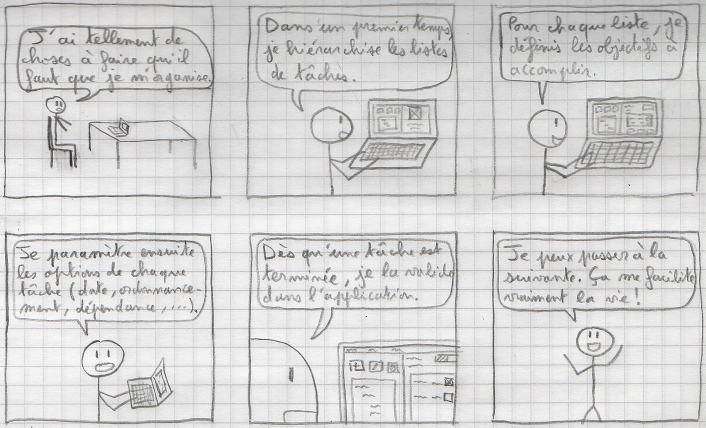
\includegraphics{img/stotyboard_ihm.png}
		   \caption{Storyboard de l'utilisation de l'application}
		\end{figure}
	
		La planche ci-dessus présente les différentes étapes d'utilisation basique du logiciel par un utilisateur lambda (son niveau de compétence n'entre pas ici en compte). Voici la liste des fonctionnalités évoquées et qui devront être présentes dans l'application finale :
		\begin{itemize}
			\item Création de listes imbriquées de tâches;
			\item Paramétrages possibles : dates relatives ou absolues, ordonnancement et dépendance des tâches;
			\item Validation des tâches et affichage de l'avancement;
			\item Sauvegarde en local des modifications effectuées.
		\end{itemize}
		
		Une fois le contexte d'utilisation cerné, il faut maintenant réaliser le prototype papier pour permettre
	
	\section{Prototype papier}
	Une \href{https://www.youtube.com/watch?v=xbLaZvgkzjQ}{vidéo sur Youtube} est accessible pour montrer le fonctionnement de l'interface du prototype papier. Le rendu vidéo est en deça de ce à quoi nous nous attendions mais nous n'avons pas eu les conditions optimales (matérielles et logicielles) de production. De plus, nous avons eu très peu de temps pour le prototypage et sommes passés rapidement au développement dès lors que nous avions une interface qui faisait consensus.
	
	TODO
	

	\section{Scénarios d'utilisation}
		Plusieurs scénarios sont envisageables dans le cadre de notre application, en voici une liste non-exhaustive :
	
		\begin{itemize}
			\item C'est la première fois que l'utilisateur teste le logiciel, il le lance et commence de zéro. Il va dans un premier temps créer les listes puis créer les tâches associées. Il peut ensuite paramétrer les dates et les dépendances. A n'importe quel moment il va pouvoir sauvegarder les informations en format xml sous le nom qu'il souhaite, et ce même s'il existe par défaut une sauvegarde automatique silencieuse. Il ne lui reste plus qu'à valider les tâches pour prendre en compte son avancement global.
			\item L'utilisateur a déjà créé un fichier précédemment : il va pouvoir charger le fichier correspondant et continuer son travail là où il en était rendu. Dans le cas où certaines tâches ou listes ne sont plus d'actualité, il est possible de les modifier ou supprimer. Lorsque l'utilisateur va vouloir quitter l'application, un message va lui demander s'il souhaite conserver les modifications ou les annuler. 
		\end{itemize}
	
	
	\section{Évaluation du prototype}
		Pour avoir un point de vue extérieur, nous avons demandé à un étudiant (qui a souhaité gardé l'anonymat) de nous donner son avis sur le prototype papier. TODO
		On a demandé à Péneau ce qu'il pensait de notre paper-prototype, il a dit OK et on a modifié 2-3 trucs :)
		


\chapter{IHM}
	
	\section{Présentation}
	
		Lors de la conception de l'IHM, il nous a paru important de séparer les Listes et les Tâches afin de simplifier l'utilisation de l'application. Ainsi, le plus évident nous paraissait d'afficher d'une part les listes, et d'autre part les tâches correspondantes. 
		
		\begin{figure}[h!]
			\centering
			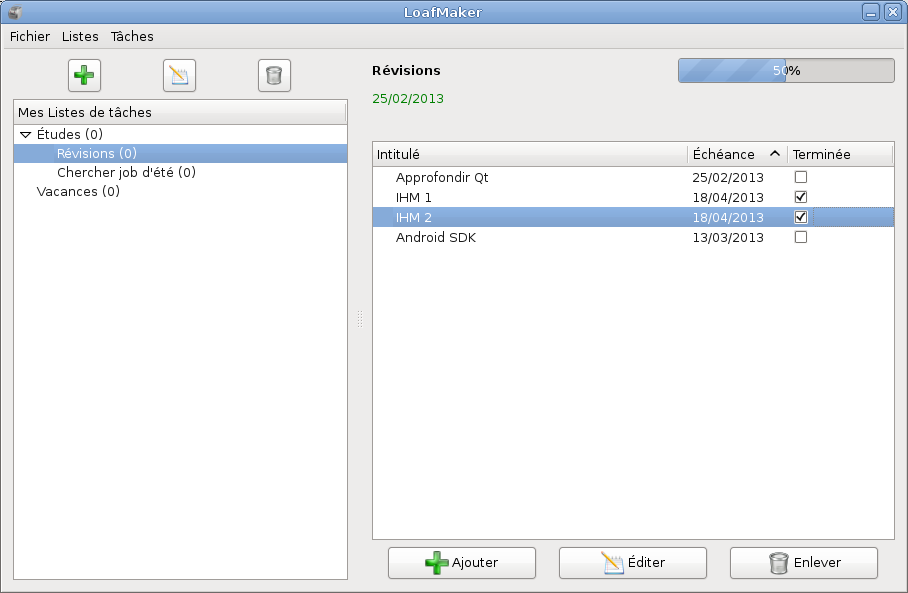
\includegraphics[scale=0.56]{mainView.png}
			\caption{Vue principale}
		\end{figure}
		\FloatBarrier
		
		Au lancement de l'application, étant donné qu'aucune liste n'est sélectionnée, le panneau de droite affichant les tâches est vide. Nous avons donc ajouté une vue de démarrage rappelant aux utilisateurs le nom de l'application et lui donnant également quelques indications pour l'aider dans sa première utilisation. Ainsi, que l'utilisateur soit néophyte ou confirmé, il ne devrait y avoir aucun problème de compréhension du logiciel.
		
		\begin{figure}[h!]
			\centering
			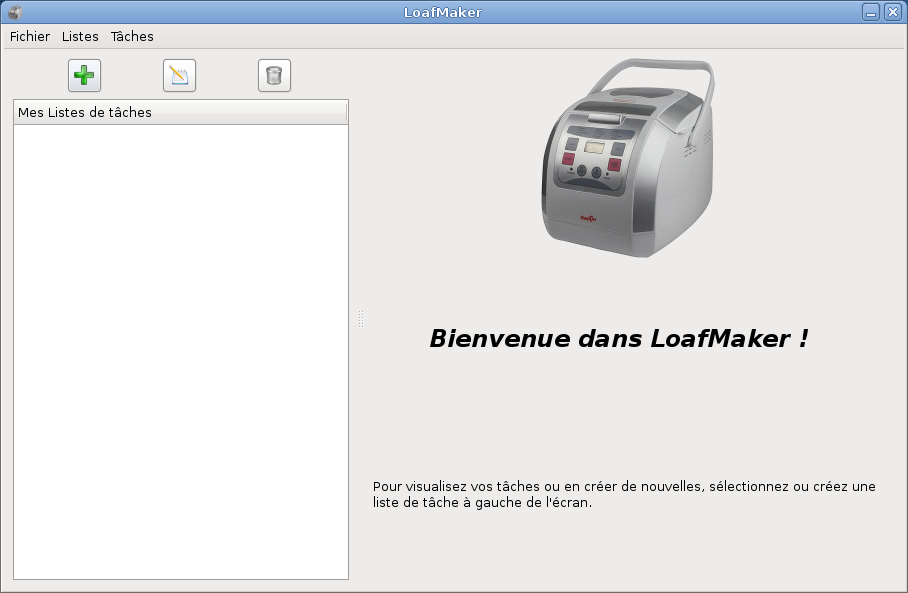
\includegraphics[scale=0.56]{startView.png}
			\caption{Vue de démarrage}
		\end{figure}
		\FloatBarrier
		
		L'ajout et la modification de listes et de tâches s'effectue en pop-up.
		
		\begin{figure}[h!]
			\centering
		 	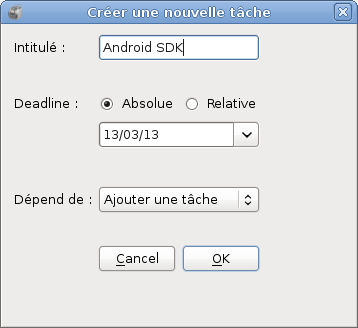
\includegraphics[scale=0.65]{newTask.png}
			\caption{Popup de demande de données}
		\end{figure}
		\FloatBarrier
		
		
		De plus, nous avons conçu l'IHM de manière à ce qu'il n'y ait aucune action de l'utilisateur qui ne soit pas associée à une réaction. Ainsi, lorsque l'utilisateur effectue une action autorisée, il peut visualiser le résultat immédiatement. S'il effectue une action interdite, il est notifié de son erreur par une popup.
		
		\begin{figure}[h!]
			\centering
		   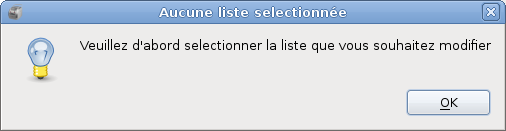
\includegraphics[scale=0.65]{popup.png}
		   \caption{Popup d'avertissement}
		\end{figure}
		\FloatBarrier
		
	
	\section{Ergonomie}
		Toute la difficulté pour la réalisation de l'interface graphique d'une telle application est de permettre de proposer à l'utilisateur néophyte un rendu clair et intuitif tout en proposant des fonctionnalités plus avancées pour un {\oe}il plus expert. Pour réussir cela, nous avons listé les différentes fonctionnalités souhaitées par ces deux groupes d'utilisateurs et les moyens possibles pour y arriver.
		
		Pour cela, nous avons décider de proposer plusieurs moyens d'arriver aux mêmes fonctionnalités. Par exemple, pour la création de tâches on peut passer par le menu de l'application, le bouton (+) sur la partie droite de l'écran, le clic droit sur cette même partie ou bien le raccourcis clavier. De cette manière, l'utilisateur aura toujours une solution qui lui conviendra plus que les autres et qu'il considèrera comme plus intuitive.
		
		De plus, nous avons choisi de toujours afficher le même menu pour ne pas perdre l'utilisateur avec des \og modes \fg d'utilisation. Ainsi, l'utilisateur aura toujours les mêmes repères visuels. Cela est important, en particulier pour les débutants, qui ne peuvent pas se raccrocher à leur expérience avec d'autres logiciels similaires.\newline
		
		Pour rendre l'utilisation plus intuitive, nous avons aussi décidé d'intégrer des icônes colorées, explicites et facilement reconnaissables pour limiter la quantité de texte à l'écran. Pour cela, nous avons utilisé des images tirées de la bibliothèque du projet \emph{Gnome}\footnote{\href{https://commons.wikimedia.org/wiki/GNOME_Desktop_icons}{Icônes disponibles ici.}} et disponibles sous licence GNU General Public License version 2. Les avantages de ces icônes sont nombreux : gratuits, libres, ergonomiques et disponibles en de nombreuses tailles, \dots \newline
		
		Nous avons souhaité permettre à l'utilisateur de contrôler dans une certaine mesure la taille des panneaux, c'est pourquoi nous avons permis d'agrandir l'un ou l'autre des côtés de la vue avec un /emph{splitter} vertical pour une meilleure lisibilité.
		
		En plus de cela, nous affichons une petite aide lors du lancement du programme pour permettre une prise en main rapide et aisée. En effet, le panneau dédié aux liste de tâche est temporairement remplacé par un message de bienvenue qui informe l'utilisateur sur le fonctionnement du logiciel.
		
		
	\section{Structure des widgets}
	
		\begin{figure}[h!]
			\centering
		   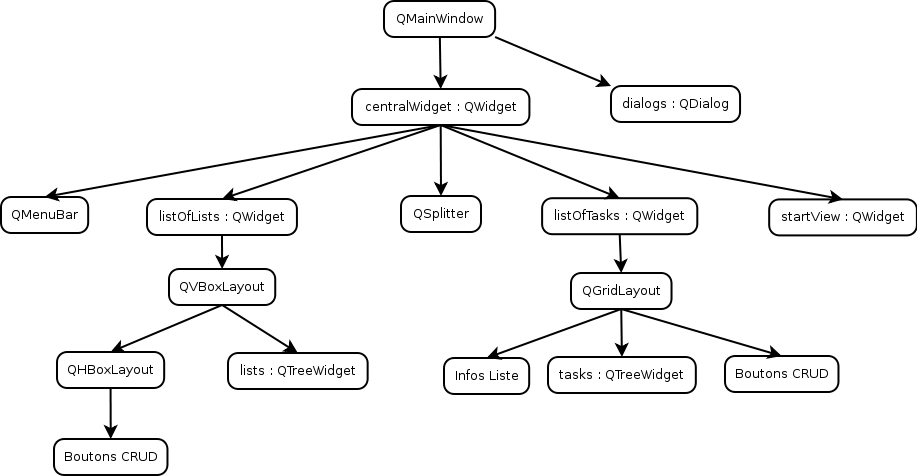
\includegraphics[scale=0.56]{struct_widget.png}
		   \caption{Structure des widgets}
		\end{figure}
		\FloatBarrier
		
		
		
	
\chapter{Limites de l'application}
	
	\section{Fonctionnalités CRUD}
	
		\begin{itemize}
			\item Lors de la suppression d'une liste, il peut arrive que l'application crash. Ce bug étant apparu assez tardivement dans le développement de l'application, nous n'avons pas eu le temps de le corriger ;
			\item Lors de la création, de la modification et de la suppression d'une liste, l'arbre des listes ne se met pas à jour correctement, et l'utilisateur est obligé de sélectionner à nouveau sa liste pour pouvoir y apporter des modifications ;
		\end{itemize}
		
		
	\section{IHM}
	
		\subsection{Fonctionnalités}
			La principale limitation que nous voyons au niveau des fonctionnalités de l'interface est l'impossibilité de redimensionner la fenêtre principale et/ou de la mettre en plein écran.
			
			Cette limitation est dûe à la présence de bugs graphiques particulièrement gênants lorsque ce redimentionnement était possible. Puisque nous voulions nous préoccuper des principales fonctionnalités en priorité, nous avons abandonné celle-ci qui ne nous semblait pas incontournable. Si nous avions bénéficié de plus de temps, cela fait partie des changements que nous aurions pu apporter.\\
			
			De plus, certaines fonctionnalités du noyau n'ont pas été implémentées côté IHM faute de temps. Ainsi, il est impossible pour l'utilisateur de spécifier une date relative, bien que nous ayons prévu son implémentation ultérieure :
			\begin{figure}[h!]
				\centering
			   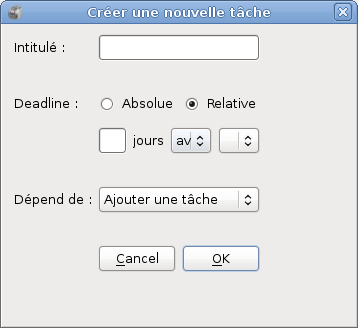
\includegraphics[scale=0.6]{newTaskRelative.png}
			   \caption{Spécification d'une tâche relative}
			\end{figure}
			\FloatBarrier
		
			De même, l'utilisateur ne peut pas spécifier de précondition à une tâche. En effet, lors de la création d'une tâche, un champ lui permet de sélectionner une tâche qui doit absolument être terminée avant celle qu'il créer. Cependant, aucun choix n'est possible puisque le champ de sélection est vide.
			
		
		\subsection{Qualité visuelle}
			Une des limites de l'application est la variation du rendu de l'interface graphique en fonction des systèmes d'exploitation ou/et des gestionnaires de fenêtres utilisés. Ce problème étant inhérent à Qt, il est cependant possible de diminuer son impact en ajoutant \og -style=cleanlooks \fg dans les options de lancement du programme. Cela permet plusieurs choses : sur certains système l'interface est plus agréable à l'{\oe}il, les fenêtres de dialogues peuvent proposer des icônes claires pour les boutons \emph{Ok} et \emph{Annuler} et cela permet d'uniformiser un peu plus les rendus. De plus, certains éléments comme le splitter, qui permet de modifier la taille des panneaux, sont plus visibles et un peu plus gros. Cela rend l'interface de l'application plus intuitive et plus explicite.
	
			Cependant, nous n'avons pas essayé notre application sur d'autres systèmes d'exploitation, nous ne garantissons pas ni son bon fonctionnement, ni l'intégrité de l'interface graphique. En revanche, les tests sur les machines du CIE ont été concluants, comme il était demandé dans le sujet du TP.\\
			
			Nous avons également rencontré quelques problèmes d'encodage que nous n'avons pas eu le temps de régler et qui affichent parfois mal les caractères spéciaux tels que les accents. Ce problème pourra être corrigé très vite ultérieurement.


\chapter{Évaluations}
	
	Utilisateurs néophytes :
		Ma mère et ma soeur
		Ta mère
		
	Utilisateurs avancés :
		Pierre-Yves
		Leroux

